\documentclass[a4paper,10pt]{article}
%\documentclass[a4paper,10pt]{scrartcl}

\usepackage[utf8]{inputenc}
\usepackage[russian]{babel}
\usepackage{graphicx}
\graphicspath{{pictures/}}
\DeclareGraphicsExtensions{.pdf,.png,.jpg}

\title{ЗАДАЧА №3. ДИФФЕРЕНЦИРОВАНИЕ}
\author{Попыкина Алёна, Козлов Александр} 
\date{12 мая 20}

\begin{document}
\maketitle
\section{Оптимизация}
    Первым делом хотелось бы уделить внимание вопросам оптимизации, и вот в чём они заключаются. Как и ранее значение корня уравнения $x \alpha = \ctg{x} $ будем вычислять методом Райдера, так как он проявил себя хорошо в прошлые разы. Но ранее представление о его <<хорошести>> было несколько поверхностным --- мы лишь знали, что этот метод даёт за 4 шага достаточно точный ответ. Методом перебора $N$ колечества шагов было найдено, что точность сохраняется и при $N = 3$ (см. рис. \ref{graph1}). То есть нам важны только первые шесть точек после запятой корня и мы их точно находим при $N = 3$.
    \begin{figure}[h]
        \noindent\centering{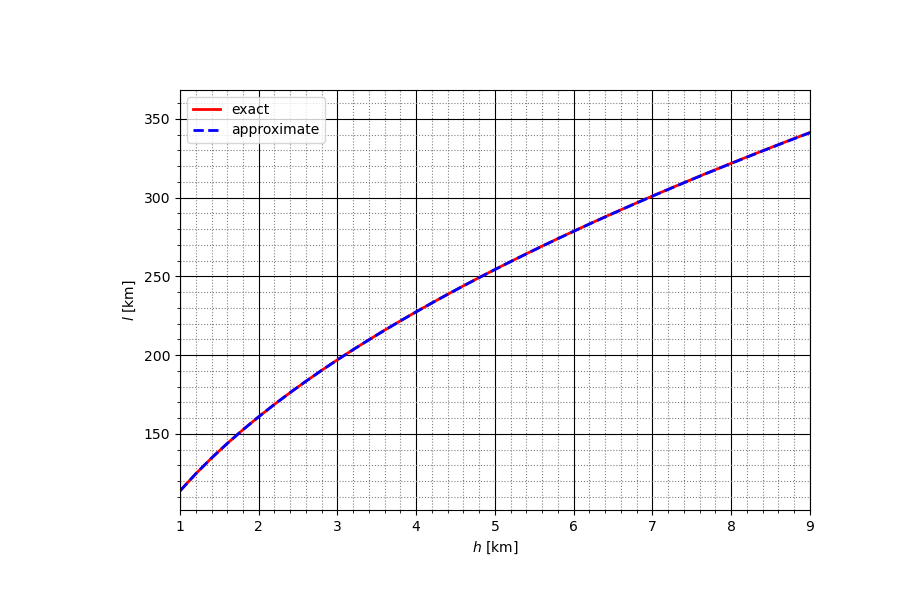
\includegraphics[width = 70mm]{1.png}}
        \caption{Вычисление ошибки корня, посчитанного с заданным количеством итераций $N$, с $x_0 = 0.860334$ --- корнем выражения, определённым ранее, при $\alpha = 1$ }
        \label{graph1}
    \end{figure} 
\section{Паде--аппроксимация}
    Самый простой способ вычисления производной в точке $\alpha = 1$ это вытащить его из Паде--аппроксимации зависимости корня от параметра $\alpha$, которая была получена ранее. Дифференцируя Паде--аппроксимацию, получаем значение $-0.313971$.\par
    Точность данного метода оценить неизвестно как, ведь порядко ошибки следует из ошибки коэффециентов Паде--аппроксимации, что не совсем тривиально, поэтому данный метод приведён для наглядности и не является основным при выполнении задания. Основными выступают следующие два метода.

\section{Производная по симметричным точкам}
    Тут всё просто. Берём и считаем разность в точке, которая на шаг $h$ остаёт от 1, и в точке, которая на шаг $h$ обгоняет 1. Получаем ответ. Его ошибка пропорциональна $h^2$.
\section{Метод Рунге--Ромберга}
    Используем трёхточечную схему Рунге--Ромберга. Так как она считает производную в $(n + \frac12)$--ой точке, то устраиваем сетку таким образом, чтобы единица оказалась на $(n + \frac12)$--ом месте. Данный метод достаточно хорош, позволяет найти ответ с точностью до куба шага.\\ То есть при шаге $0.01$ уже имеем значение, которому можно доверять вплоть до пятой цифры после запятой.
\section{Заключение}
    Наиболее точным оказался метод Рунге--Ромберга. Ещё интересным наблюдением явялется то, что дифференцирование Паде--аппроксимации дало ответ, близкий к методу Рунге--Румберга --- они совпадают до пятой цифры после запятой. При уменьшении шага результат метода дифференцирования по симметричным точкам приблизился к тому, что выдаёт Рунге--Румберг.
\begin{figure}[h]
\begin{minipage}[h]{0.6\linewidth}
\center{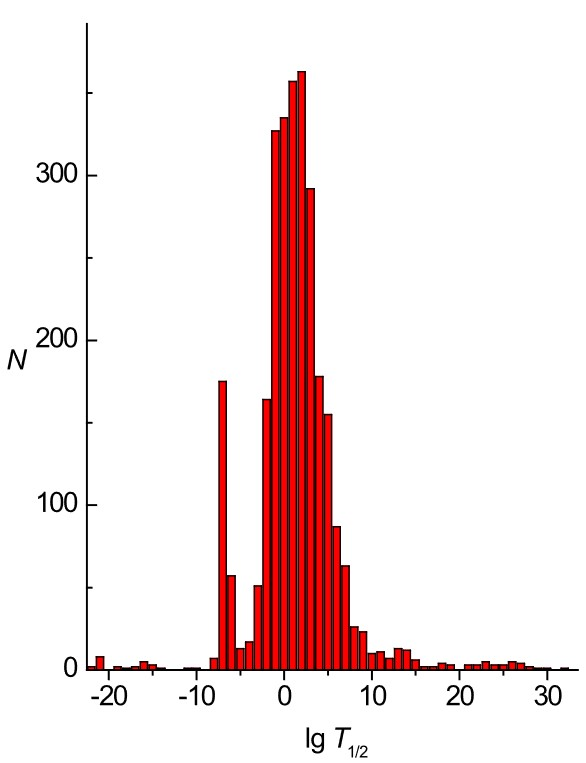
\includegraphics[width=1.1\linewidth]{2.png} \\ а)}
\end{minipage}
\hfill
\begin{minipage}[h]{0.6\linewidth}
\center{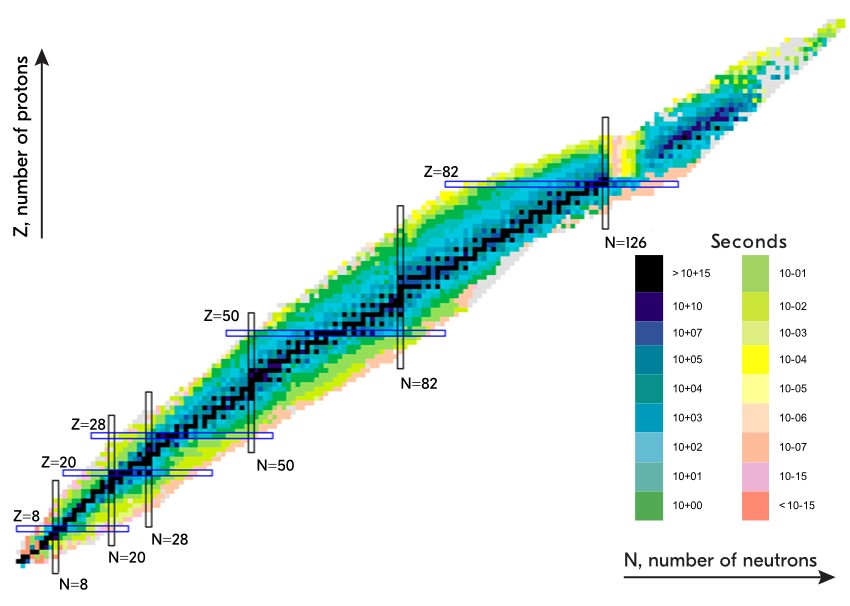
\includegraphics[width=1\linewidth]{3.png} \\ б)}
\end{minipage}
\caption{Результат работы программы}
\label{ris:image1}
\end{figure}
    
\end{document}
